% define documentclass i.e. article, book, scrartcl
\documentclass[11pt, a4paper]{article}
\usepackage[ngerman, english]{babel}

% figure usepackages
\usepackage{graphicx}
\usepackage{float}
\usepackage{caption}
\usepackage{subcaption}

% differnet encoding i.e. UTF-8 ISO-8859-1
\usepackage[utf8]{inputenc}

% math usepackages
\usepackage{amsmath}
\usepackage{amssymb}
\usepackage{amsfonts}
\usepackage{eurosym}

% hyperlinks
\usepackage{hyperref}

% to-do-notes (\todo{Do this do that}) - \listoftodos
\usepackage{todonotes}

% page margins and spacing
\usepackage[margin=2cm, nohead]{geometry}
\usepackage[onehalfspacing]{setspace}

% table usepackages
\usepackage{array}

% list usepackages
\usepackage{lmodern}

% code usepackages
\usepackage{listings}
\usepackage[framed,numbered,autolinebreaks,useliterate]{mcode}

% font usepackages
\usepackage{ae, aecompl}
\usepackage[T1]{fontenc}
\usepackage{anyfontsize}
\usepackage{color}

% macro usepackage
\usepackage{xparse}
\DeclareDocumentCommand{\pder}{ O{} O{} m }{\frac{\partial^{#2}#1}{\partial#3^{#2}}}

\begin{document}

\title{LateX Template for Beginners}
\author{Sascha Bilert}
\date{\today}
\maketitle
\thispagestyle{empty}
\tableofcontents

\pagebreak

\pagenumbering{arabic}

\section{Introduction}

This document is created as a Template for Latex by Sascha Bilert. I tried to implement the most frequently latex packages I use. If you have any comments please contact me under:

\href{mailto:sascha.bilert@student.jade-hs.de}{sascha.bilert@student.jade-hs.de}\\
In many cases you need to add different \textbackslash use-packages to format your Latex document for your own purpose. My goal was to build a bridge between the packages and the usage for my studentcolleges. Also i wanted to work with a git repository as a version control system for my Latex document using \textbf{.gitignore}.

So on one hand its a training for my Latex skills and on the other hand every can have a lot and maybe find some interesting aspects. I also like to mention, that i hate those {\color{blue}blue} and {\color{red}red} messages in the LOG FILE!

I usually work with \textbf{texmaker} but as you know, there a many different typesetting programmes for Latex. The latest i tried to work with is the vim editor with a Latex compiler.

\section{Section}

Here you can see different sections and subsections to arrange your information and you can have some fun with numberics or alphabetics

\subsection{First Subsection}

\subsection{Second Subsection}

\subsubsection{First Sub-Subsection}

\subsubsection{Second Sub-Subsection}

\section{Using Macros}

\section{Bullets and enumerations}

In the following section i what to say something about bullet-lists and enumerations. I don't us both very often, but in some cases its clever to know how you work with them.

\begin{itemize}
	\item First Item
	\item Second Item
		\begin{itemize}
			\item First sub-item
			\item Second sub-item
		\end{itemize}
\end{itemize}

\begin{enumerate}
	\item First statement
	\item Second statement
		\begin{enumerate}
			\item First sub-statement
			\item Second sub-statement
		\end{enumerate}
\end{enumerate}

\section{Mathematics}

\section{Figures}

\begin{figure}[H]
	\centering
	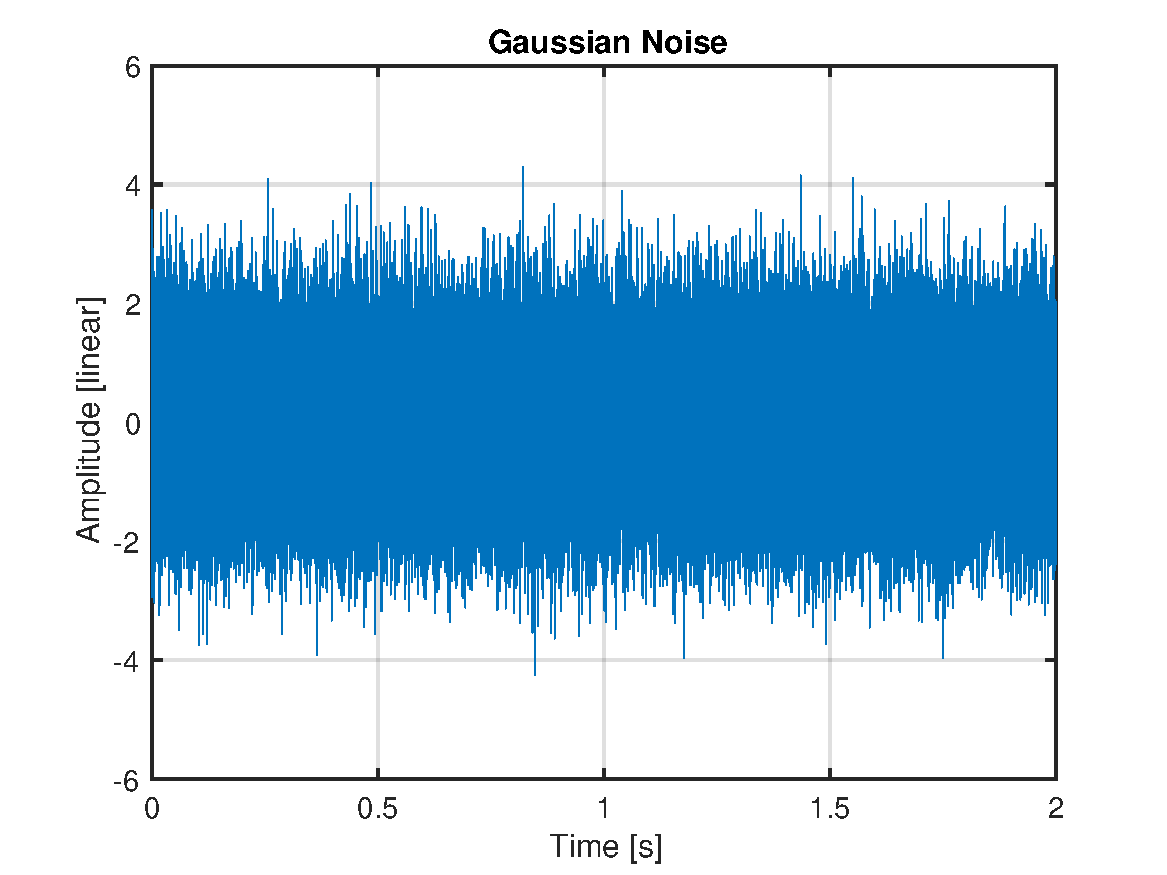
\includegraphics[scale=0.6]{plot_Template.pdf}
	\caption{Gaussian noise with $fs = 48$ kHz}
	\label{fig:image1}
\end{figure}

\section{Code-lines}

\section{Notes}

\section{The Bibliography}

This is how you do citation in LateX using different styles \cite{holube2010development} and here is another Book \cite{yost2013hearing} and some more articles \cite{verhey1999within}. We also have some in-collections \cite{bitzer2001superdirective}.

\bibliographystyle{alpha}

\bibliography{Template}

\end{document}

